\documentclass{article}
\usepackage[UTF8]{ctex}
\usepackage[tc]{titlepic}
\usepackage{titlesec}
\usepackage{cite}
\usepackage{amsmath}
\usepackage{amssymb}
\usepackage{amsfonts}
\usepackage{paralist}
\usepackage{geometry}
\usepackage{listings}
\usepackage{fancyhdr}
\usepackage{booktabs}
\usepackage{graphicx}
\usepackage{listingsutf8}
\usepackage{graphicx}
\usepackage{geometry}
\usepackage{xcolor}
\definecolor{codegreen}{rgb}{0,0.6,0}
\definecolor{codegray}{rgb}{0.5,0.5,0.5}
\definecolor{codepurple}{rgb}{0.58,0,0.82}
\definecolor{backcolour}{rgb}{0.95,0.95,0.92}
\lstset{
	basicstyle          =   \ttfamily,          % 基本代码风格
	keywordstyle        =   \bfseries,          % 关键字风格
	commentstyle        =   \rmfamily\itshape,  % 注释的风格,斜体
	stringstyle         =   \ttfamily,  		% 字符串风格
	xleftmargin         =   -10pt,
	flexiblecolumns,                
	numbers             =   left,   			% 行号的位置在左边
	showspaces          =   false,  			% 是否显示空格,显示了有点乱,所以不现实了
	numberstyle         =   \zihao{-5}\ttfamily,% 行号的样式,小五号,tt等宽字体
	showstringspaces    =   false,
	captionpos          =   t,      			% 这段代码的名字所呈现的位置,t指的是top上面
	frame               =   lrtb,   			% 显示边框
}

\lstdefinestyle{C}{	
	language        =   C, 				
	basicstyle      =   \zihao{-5}\ttfamily,
	numberstyle     =   \zihao{-5}\ttfamily,
	keywordstyle    =   \color{blue},
	keywordstyle    =   [2] \color{teal},
	stringstyle     =   \color{magenta},
	commentstyle    =   \color{red}\ttfamily,
	breaklines      =   true,   				
	columns         =   fixed,  			
	% basewidth       =   0.5em,
}
\lstdefinestyle{mystyle}{
	backgroundcolor=\color{backcolour},   
	commentstyle=\color{codegreen},
	keywordstyle=\color{magenta},
	numberstyle=\tiny\color{codegray},
	stringstyle=\color{codepurple},
	basicstyle=\ttfamily\footnotesize,
	breakatwhitespace=false,         
	breaklines=true,                 
	captionpos=b,                    
	keepspaces=true,                 
	numbers=left,                    
	numbersep=5pt,                  
	showspaces=false,                
	showstringspaces=false,
	showtabs=false,                  
	tabsize=2
}
\lstset{
	basicstyle=\ttfamily,
	keywordstyle=\color{blue}\bfseries,
	commentstyle=\color{gray},
	breaklines=true,
	columns=fullflexible,      % 关键:允许中文断行显示
	keepspaces=true,
	escapeinside={}{},       % 支持插入 LaTeX 指令
	extendedchars=false  ,     % 不要使用 extended characters
	inputencoding=utf8,      
}


\usepackage[section]{placeins}
\geometry{a4paper,scale=0.8}
\pagestyle{fancy}

\usepackage{ctex}
\usepackage{CJKutf8}


\lhead{大气污染物扩散的粒子追踪\\\today}
\chead{中国科学技术大学\\数学建模课程}

\rhead{Assignment x\\ {\CTEXoptions[today=old]\today}}
\newcommand{\upcite}[1]{\textsuperscript{\cite{#1}}}

\titleformat*{\section}{\bfseries\Large}
\titleformat*{\subsection}{\bfseries\large}

\title{\bfseries 大气污染物扩散的粒子追踪}
\author{
	梅振源 \quad  71 \quad PB22030795\\
	侯维铭  \quad  64\quad PB22010431\\
	苏睿涵  \quad 15 \quad PB22000078
}

\begin{document}
	\maketitle
	\begin{abstract}
		随着工业化进程加快,大气污染物(如PM2.5)的扩散规律受到越来越多关注。特别是在复杂地形和特殊气象条件下,污染物的传输特征亟待研究。事实上,这是一个复杂的过程,涉及到风场,湍流,地形,热力学等多种因素的影响。本文旨在构建含拉格朗日粒子模型,对数风廓线模型与高斯烟羽模型在内的多种模型。基于Matlab软件,结合全球地形数据,考虑涡旋风场,匀速风场,山地地形等多种不同的其余因素追踪模拟粒子扩散。根据模拟结果比对,发现拉格朗日模型可以更好的适应动态过程,相较于高斯烟羽模型能更好地模拟复杂的风场与地形变化,进行非均匀扩散,但相应的计算量要求较高,而高斯烟羽模型模拟的是稳态和均匀风场下的污染物呈现高斯分布的烟羽状,牺牲对复杂动态过程的刻画能力换取了相对较小的计算量。结合多种模型,模拟结果显示:在旋转风场作用下,污染物呈螺旋状扩散;在匀速风场作用下,污染物呈烟羽状;复杂地形显著影响粒子沉积分布,沉积主要集中于地势高差较大的区域等。本研究有助于理解污染物在环境中的迁移机制,并为环境治理和灾害预警提供参考。
	\end{abstract}
	\clearpage
	
	\setcounter{section}{2}
	\section*{\centerline{一、前言}}
	
	随着城市迅速发展,人类活动排放的空气污染物种类和数量不断增加,其中以PM2.5为代表的细颗粒物因其对人体健康和生态环境的严重影响而受到广泛关注。准确模拟和预测污染物在大气中的扩散规律,已成为一个重要研究课题。\\
	\indent 污染物在大气中的传输扩散过程受多种因素影响,包括风场结构、湍流强度、地形起伏以及大气热力稳定度等。这一过程具有高度的非线性和不确定性,因此,建立合理的扩散模型成为研究污染物扩散机制的关键。\\
	\indent 目前常用的扩散模型主要包括高斯烟羽模型与拉格朗日粒子模型。高斯烟羽模型由于计算简便、物理含义清晰,广泛用于污染物在匀速风场和稳态条件下的估算。但该模型假设较强,难以适应非稳态、非均匀风场或复杂地形条件下的模拟。而拉格朗日粒子模型则通过追踪大量粒子在风场与扩散场中的运动轨迹,能够灵活地处理不规则边界、非均匀风速和瞬态过程,具有更高的精度和适应性。\\
	\indent 本文旨在比较两种模型在不同气象与地形条件下模拟PM2.5扩散的性能差异。我们基于MATLAB平台,结合全球地形数据构建了具备旋转风场、匀速风场与真实地形条件的模拟系统,分别实现了高斯烟羽模型与拉格朗日粒子模型的扩散模拟。在对比模拟结果的基础上,分析了风场结构、地形起伏对污染物分布形态与沉积分布的影响,为后续的污染源追踪提供理论支持和参考。
	
	
	
	\section*{\centerline{二、模型的原理与建立}}
	\subsection{拉格朗日粒子模型}
	拉格朗日模型的考虑对象是每个污染物粒子的扩散轨迹,它认为每个粒子的运动轨迹都遵从下面的随机微分方程描述:
	\[ \dfrac{d\vec{X}}{dt}=\vec{U}(\vec{X},t)+\vec{R}(t) \]
	其中
	\begin{itemize}
		\item $ \vec{X}=(x,y,z)$表示粒子在$t$时刻所处的位置向量
		\item $\vec{U}(\vec{X},t)=(u_x,u_y,u_z)$表示$ t$时刻$\vec{X}$位置的环境风场
		\item $\vec{R}(t) $表示$t$时刻湍流扰动
	\end{itemize}
	
	
	\indent 湍流扰动$\vec{R}(t) $一般采用随机游走模型:
	\[ \vec{R}(t)=\dfrac{d\vec{X_d}}{dt}=\dfrac{\sqrt{2K}dW(t)}{dt} \]
	其中
	\begin{itemize}
		\item $ K=(K_x,K_y,K_z)$是扩散系数,每项单位通常是$m^2/s$,表示单位时间内粒子运动扩散的强度
		\item $W(t)$表示三项独立的标准布朗运动
	\end{itemize}
	
	
	结合可知
	\begin{align*}
		d\vec{X}&=\vec{U}(\vec{X},t)dt+\vec{R}(t)dt\\
		&= \vec{U}(\vec{X},t)dt+\sqrt{2K}dW(t)\\
		&=\vec{U}(\vec{X},t)dt+\sqrt{2Kdt}R
	\end{align*}
	\begin{itemize}
		\item $R=(R_x,R_y,R_z)$表示三向独立的标准正态分布
	\end{itemize}
	
	
	也即
	\begin{align*}
		\Delta x&= \vec{U}(\vec{X},t)\Delta t+\sqrt{2K\Delta t}R\\
		\vec{X}_{t+\Delta t}&=\vec{X}_t  + \vec{U}(\vec{X},t)\Delta t+\sqrt{2K\Delta t}R
	\end{align*}
	
	
	根据经验结论$K$各个分量均可以取$0.4$,因此只要给出风场条件和粒子坐标,我们可以容易地利用这个模型给出粒子运动预测
	
	\subsection{高斯烟羽模型}
	高斯烟羽模型的核心公式如下:
	\[
	C(x, y, z) = \frac{Q}{2\pi u \sigma_y \sigma_z} 
	\exp\left( -\frac{y^2}{2\sigma_y^2} \right) 
	\left(
	\exp\left( -\frac{(z - H)^2}{2\sigma_z^2} \right)
	+ 
	\exp\left( -\frac{(z + H)^2}{2\sigma_z^2} \right)
	\right)
	\]
	其中
	\begin{itemize}
		\item $C(x,y,z)$表示污染物在$(x,y,z)$处的浓度,单位为$g/m^3$
		\item $Q$为源强,单位为$g/m$
		\item $u$为风速,单位为$m/s$
		\item $H$为有效排放距离,单位为$m$
		\item $ \sigma_y,\sigma_z $为扩散系数,表示在横向和纵向的标准差
		\item $x$为下风方向距离,单位为$m$
		\item $y$横线偏移距离,单位为$m$
		\item $z$垂直高度,单位为$m$
	\end{itemize}
	
	
	\indent 	特别的,对于其中的扩散系数$ \sigma_y,\sigma_z $有如下经验公式:
	\[ \sigma_y(x)=ax^b\hspace{1em} ,\hspace{1em} \sigma_z(x)=cx^d\]
	\indent 具体$a,b,c,d$依据大气等级而定,为了更快的扩散速率以便观察,我们可以取$a=c=0.5,b=d=0.8$。\\
	\indent 需要注意的是$H$并不等同于源的高度,实际上由于烟喷出时的动能,和烟气温度高于周围气体产生的密度差,使得烟气有效排放高度会提升一段距离,这就是烟气抬升效应。这里我们考虑的是静态的情况,温差产生的浮力抬升占据主导,动能抬升的影响忽略。\\
	\[ H=H_0+\Delta H \]
	\indent 根据Briggs经验公式
	\begin{align*}
		F_b&=gv_s(\frac{d}{2})^2\dfrac{T_g-T_a}{T_g}\\
		\Delta H &= 
		\begin{cases}
			38.7 \dfrac{F_b^{3/5}}{u_0 \, s^{1/5}}, & F_b > 55 \\[8pt]
			21.4 \dfrac{F_b^{3/4}}{u_0}, & F_b \leq 55
		\end{cases}\\
		x_f &= 
		\begin{cases}
			119 \, F_b^{2/5}, & F_b > 55 \\[8pt]
			49 \, F_b^{5/8}, & F_b \leq 55
		\end{cases}
	\end{align*}
	
	
	结合上面的公式即可用高斯烟羽模型模拟稳态情况下的扩散情况。
	\subsection{其余细节}
	除去拉格朗日粒子模型和高斯烟羽模型,我们还尝试了加入一些其他模型,例如用对数风廓线模型刻画风速$u$随着高度$z$的变化 :
	\[ u(z)=\dfrac{u_*}{\kappa}ln(\dfrac{z-d}{z_0}) \]
	其中
	\begin{itemize}
		\item $u_*$表示磨擦速度,反映地表剪切应力大小,单位为$m/s$
		\item $\kappa$是von Kármán常数,可取$0.4$
		\item $d$是地表障碍物高度,一般取$0$即可
		\item $z_0$表示地面粗糙度长度,单位为$m$
	\end{itemize}
	\indent 考虑到$u_*$的求解并不容易,我们通过给定某处的风速进行推算,例如如果给定了$z_{ref}$处的风速$u_{ref}$,那么有
	\[ u_* = \frac{u_{\text{ref}} \cdot \kappa}{\ln\left( \frac{z_{\text{ref}}}{z_0} \right)}
	\]
	\indent 那么原公式就等价于
	\[ u(z) = u_{\text{ref}} \cdot \frac{\ln\left(\dfrac{z}{z_0}\right)}{\ln\left(\dfrac{z_{\text{ref}}}{z_0}\right)}
	\]
	\indent 这就变成了容易的形式。\\
	\indent 此外拉格朗日模型部分中,当粒子接触到地面,我们假设他会以适当比例沉积与反弹,这部分并无特别公式模型,故不再赘述。
	
	\setcounter{section}{3}
	\setcounter{subsection}{0}
	\section*{\centerline{三、程序的实现}}
	\addcontentsline{toc}{section}{三、程序的实现}
	\subsection{考虑对数风廓线的拉格朗日模型}
	我们采用正弦波来模拟坡度较小的平缓地面。
	\begin{lstlisting}
		A1 = 300; f1 = 0.0001;   
		A2 = 200; f2 = 0.0003;  
		terrain = @(x,y) A1 * sin(2*pi*f1*x) .* sin(2*pi*f1*y) + ...
		A2 * sin(2*pi*f2*x) .* sin(2*pi*f2*y);\end{lstlisting}
	\indent 根据风廓线模型进行风速计算的关键步骤如下,具体公式变形原理前面已经解释,此处不再赘述:
	\begin{lstlisting}
		u_local = (u_ref * log(max(h_above_ground, z0+0.01)/z0)) / log(z_ref/z0);
		v_local = zeros(numActive, 1);
		w_local = zeros(numActive, 1);\end{lstlisting}
	\indent 接着通过拉格朗日模型公式和求解出的风速对每个粒子的位置进行更新。
	\begin{lstlisting}
		dx = u_local * dt + sqrt(2*Kx*dt) * randn(numActive, 1);
		dy = v_local * dt + sqrt(2*Ky*dt) * randn(numActive, 1);
		dz = w_local * dt + sqrt(2*Kz*dt) * randn(numActive, 1);
		
		particles(active_idx, 1) = active_particles(:,1) + dx;
		particles(active_idx, 2) = active_particles(:,2) + dy;
		particles(active_idx, 3) = active_particles(:,3) + dz;\end{lstlisting}
	\indent 由于此处的假设地形坡度较低,我们假设粒子与地面碰撞后会完全沉积,并在后续可视化操作中对乘沉积的粒子进行特殊标色。
	\begin{lstlisting}
		for i = find(active_idx)'
		x = particles(i, 1);
		y = particles(i, 2);
		terrain_height = terrain(x, y);
		if particles(i, 3) < terrain_height
		absorbed(i) = true;
		end
		end\end{lstlisting}
	\subsection{涡旋风场下的拉格朗日模型}
	\indent 这里我们选择使用matlab自带的全球地形数据topo截取一段山地地形进行模拟,并且假设自然环境中有着涡旋风场。\\
	\indent 先设定涡旋风场的基本参数
	\begin{lstlisting}
		vortex_center = [500000, 500000];  % 距涡旋中心500km
		vortex_strength = 5e6;             % 涡旋强度 (<1000km)
		max_wind_speed = 20.0;             % 最大风速 (m/s)
		wind_direction = 1;                % 1逆时针, -1顺时针
		Kx = 100; Ky = 100; Kz = 10;       % 扩散系数 \end{lstlisting}
	\indent 接着计算旋转风场函数
	\begin{lstlisting}
		function [u, v, w] = vortex_velocity(x, y, vortex_center, vortex_strength, ...
		max_wind_speed, wind_direction)
		dx = x - vortex_center(1);
		dy = y - vortex_center(2);
		r = sqrt(dx.^2 + dy.^2);
		r(r < 1000) = 1000;  % 避免中心处奇异值
		
		% 计算切向速度
		tangential_velocity = vortex_strength ./ r;
		tangential_velocity = min(tangential_velocity, max_wind_speed);
		
		u=-wind_direction*tangential_velocity.*dy./r;
		v=wind_direction*tangential_velocity.*dx./r;
		
		% 垂直风速 
		w = zeros(size(x));
		center_distance=r;
		w(center_distance<200000)=0.5*...
		(1-center_distance(center_distance < 200000)/200000);
		end\end{lstlisting}
	\indent 周期更新粒子位置
	\begin{lstlisting}
		[u_local, v_local, w_local] = vortex_velocity(... 
		active_particles(:,1), active_particles(:,2), ...
		vortex_center, vortex_strength, max_wind_speed, wind_direction);
		
		dx = u_local * dt + sqrt(2*Kx*dt) * randn(numActive, 1);
		dy = v_local * dt + sqrt(2*Ky*dt) * randn(numActive, 1);
		dz = w_local * dt + sqrt(2*Kz*dt) * randn(numActive, 1);
		
		particles(active_idx, 1) = active_particles(:,1) + dx;
		particles(active_idx, 2) = active_particles(:,2) + dy;
		particles(active_idx, 3) = active_particles(:,3) + dz;
	\end{lstlisting}
	\indent 特别的是由于风速较快与地形坡度较大,此处我们假设碰撞到地面的粒子有$10\% $的概率进行反弹,不会静止而是将高度反向抬升后继续运动
	\begin{lstlisting}
		for i = find(active_idx)'
		x = particles(i, 1);
		y = particles(i, 2);
		terrain_height = terrain(x, y);
		if particles(i, 3) < terrain_height
		if rand < 0.9
		absorbed(i) = true;
		deposit_time(i) = t;
		deposit_position(i, :) = [x, y, terrain_height];
		else 
		rebounded(i) = true;
		particles(i,3) = terrain_height + 10; % 反弹10米高度
		end
		end
		end\end{lstlisting}
	\subsection{稳态下的高斯烟羽模型}
	\indent 高斯烟羽模型相较于拉格朗日模型没有复杂的粒子运动过程,而是稳态下的浓度分布,这一部分公式如下:
	\begin{lstlisting}
		term1 = exp(-(Y.^2)./(2*sig_y.^2));
		term2 = exp(-(Z - H_eff_grid).^2./(2*sig_z.^2)) + ...
		exp(-(Z + H_eff_grid).^2./(2*sig_z.^2));
		C = Q0./(2*pi*u0.*sig_y.*sig_z) .* term1 .* term2;\end{lstlisting}
	\indent 其中烟气抬升部分也分类较为繁琐且并非核心部分,此处也不再赘述。\\
	为了更直观地看到浓度分布,我们截取了部分截面与切面,在结果部分进行展示。
	\newpage
	\setcounter{section}{4}
	\setcounter{subsection}{0}
	\section*{\centerline{四、结果}}
	\subsection{考虑对数风廓线的拉格朗日模型}
	\begin{figure}[htbp]
		\centering
		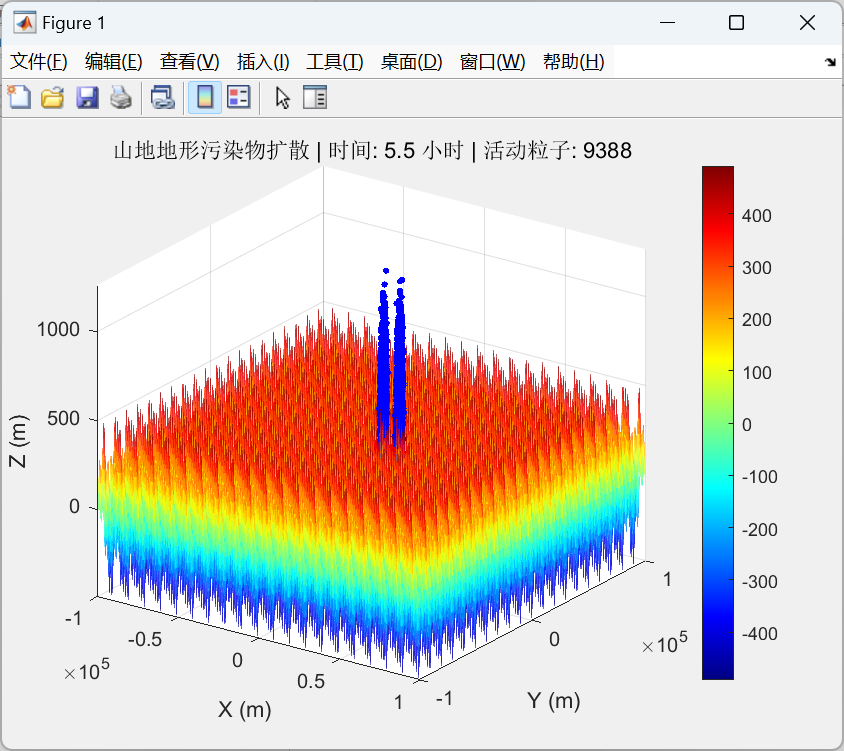
\includegraphics[width=8cm]{Logarithmic wind profile1.png}
		\caption{扩散前期分布图}
		\label{fig:your_label}
	\end{figure}
	\FloatBarrier
	\begin{figure}[htbp]
		\centering
		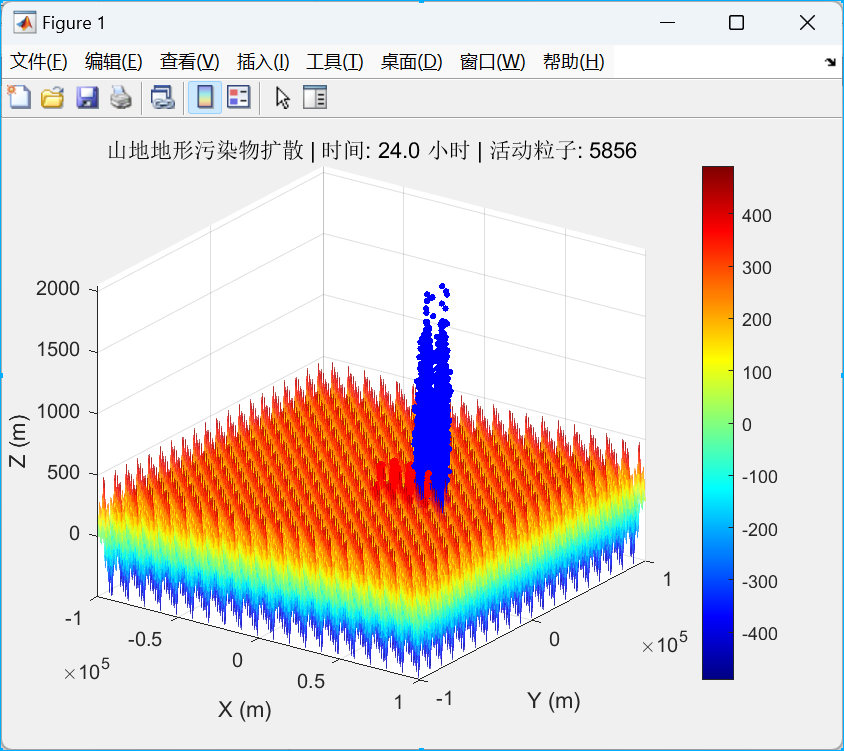
\includegraphics[width=8cm]{Logarithmic wind profile2.png}
		\caption{扩散后期分布图}
		\label{fig:your_label}
	\end{figure}
	\FloatBarrier
	\begin{figure}[htbp]
		\centering
		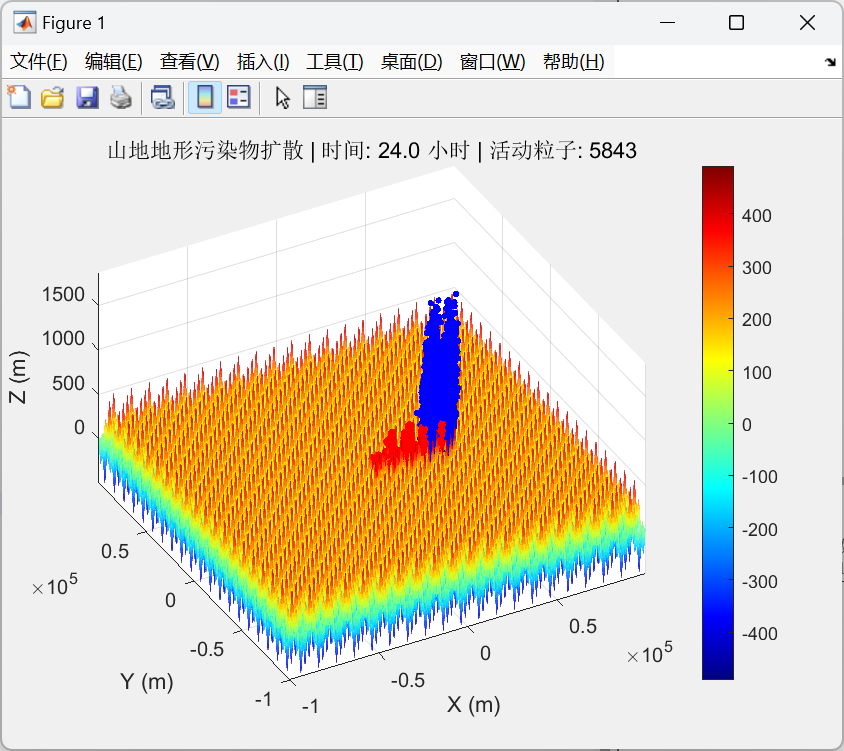
\includegraphics[width=8cm]{Logarithmic wind profile3.png}
		\caption{扩散后期分布图2}
		\label{fig:your_label}
	\end{figure}
	\FloatBarrier
	\subsection{涡旋风场下的拉格朗日模型}
	\FloatBarrier
	\begin{figure}[htbp]
		\centering
		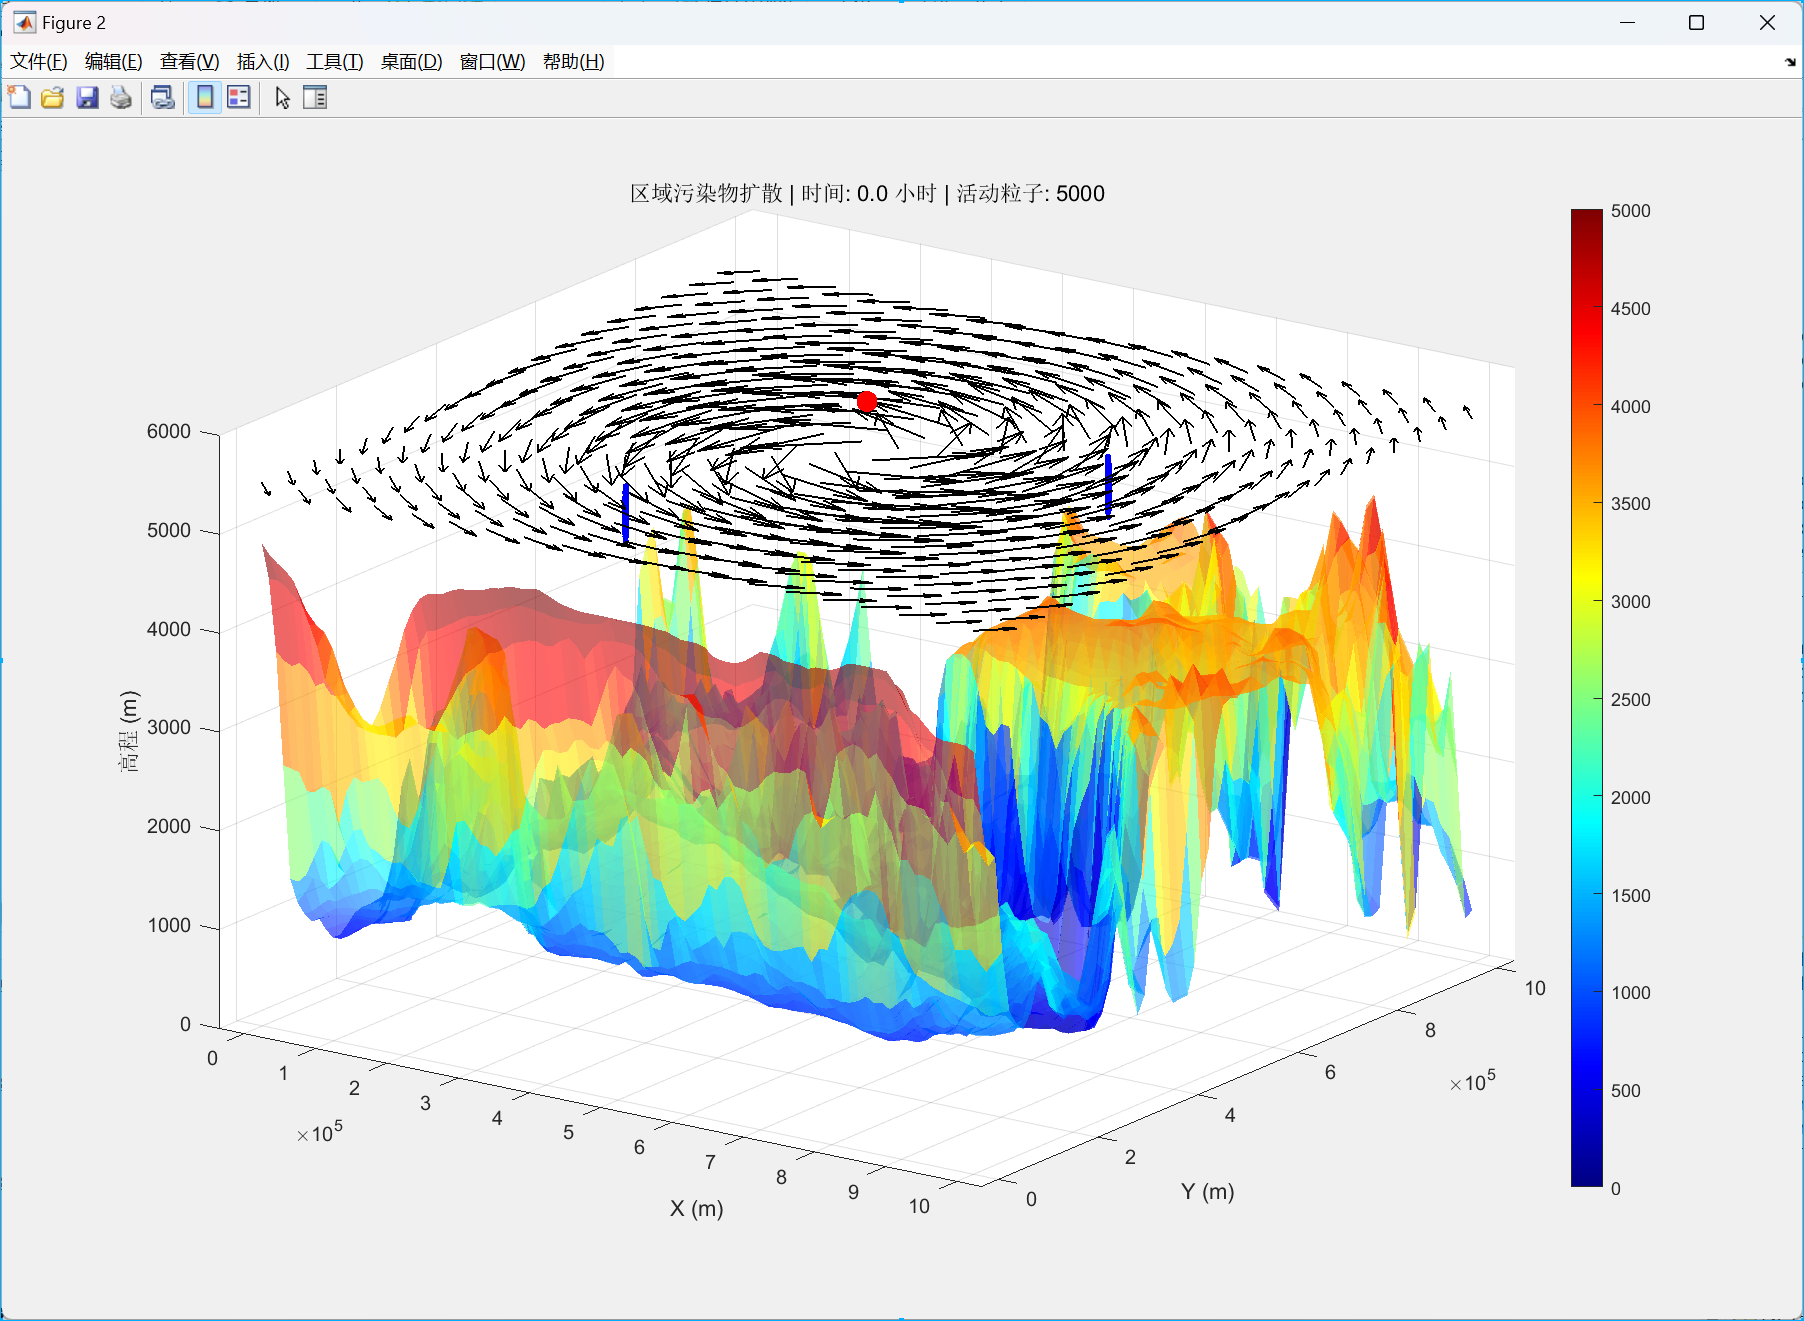
\includegraphics[width=10cm]{Lagrange1.png}
		\caption{扩散前期分布图}
		\label{fig:your_label}
	\end{figure}
	\FloatBarrier
	\begin{figure}[htbp]
		\centering
		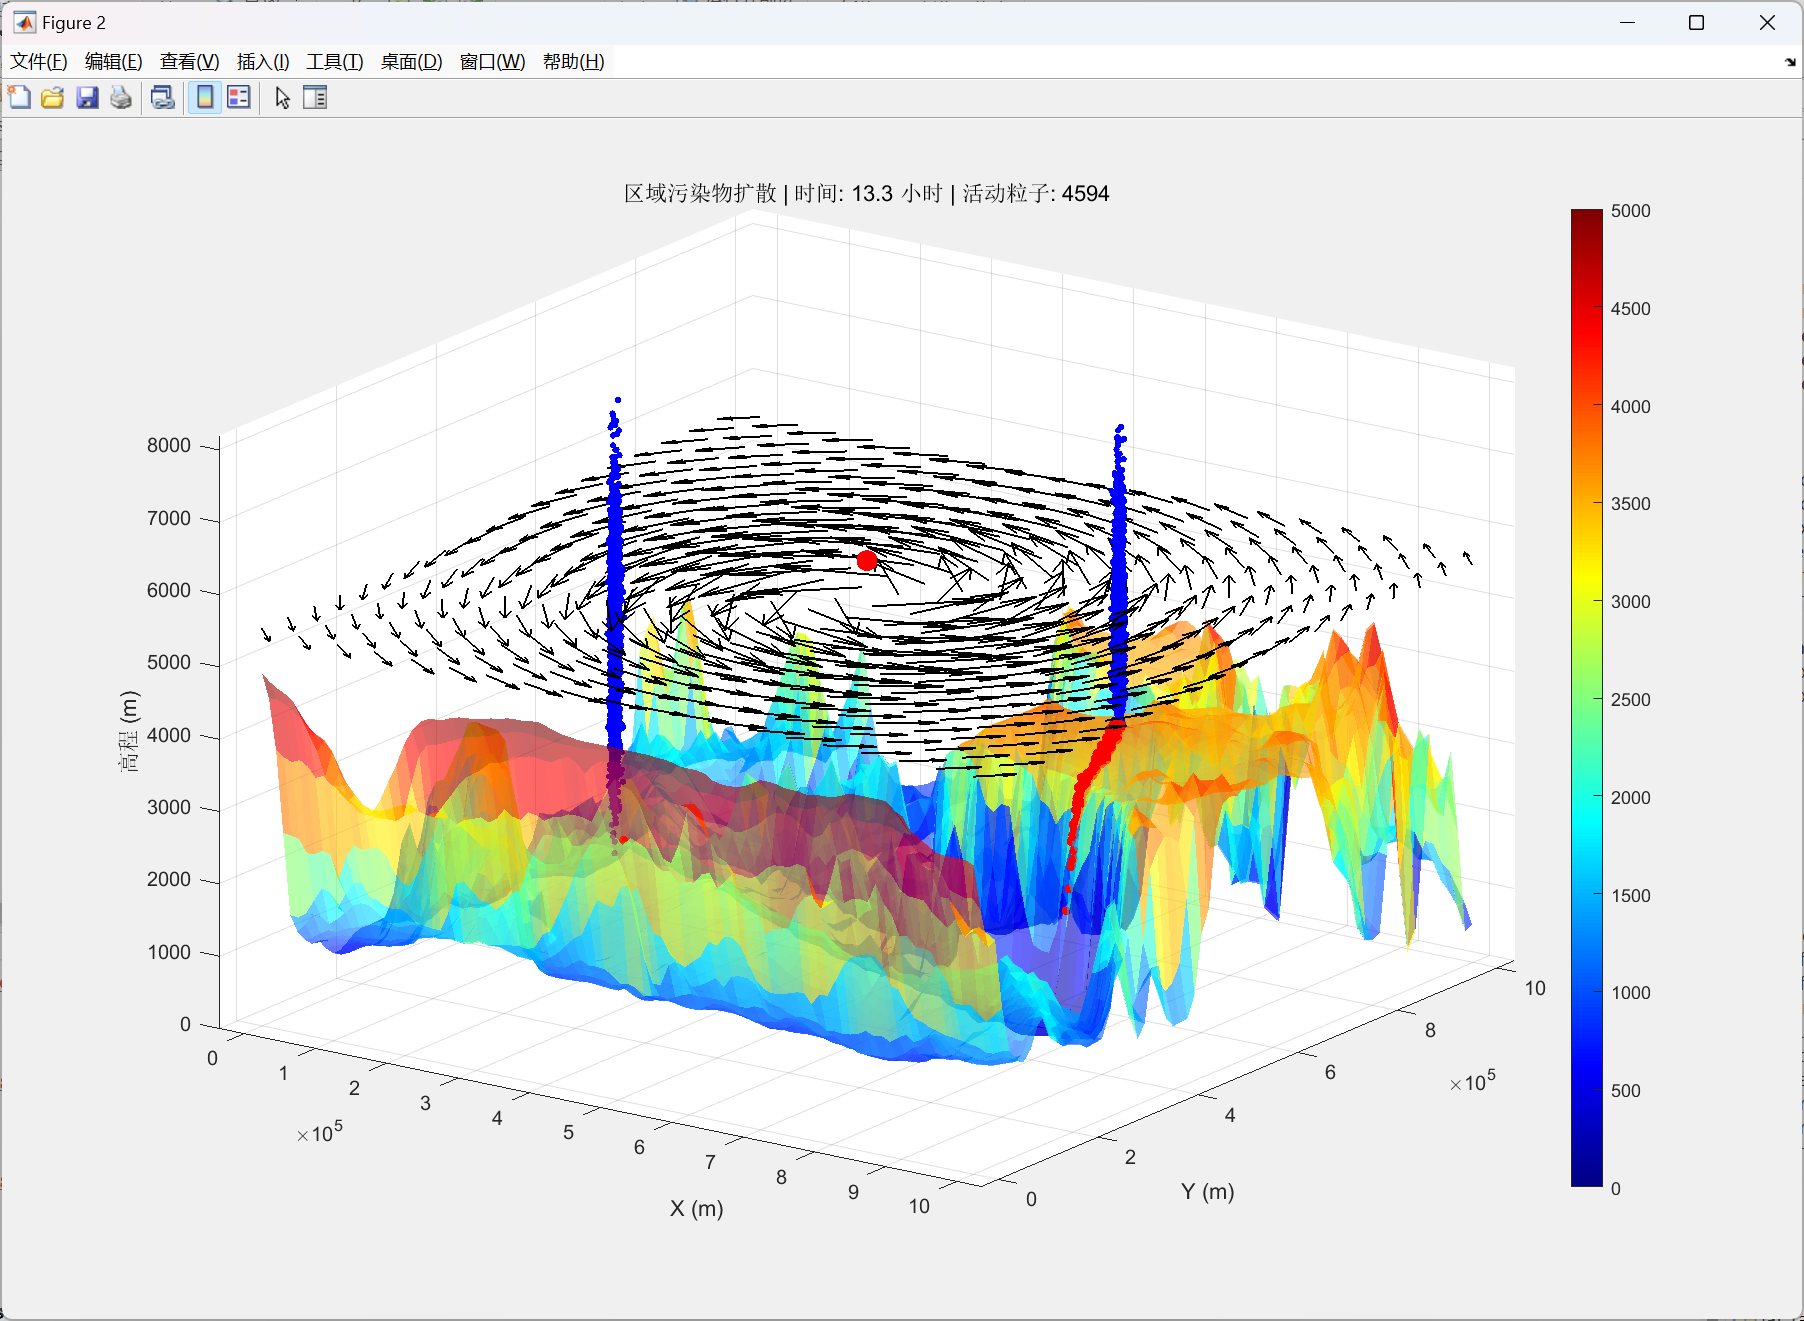
\includegraphics[width=10cm]{Lagrange2.png}
		\caption{扩散后期分布图}
		\label{fig:your_label}
	\end{figure}
	\FloatBarrier
	\begin{figure}[htbp]
		\centering
		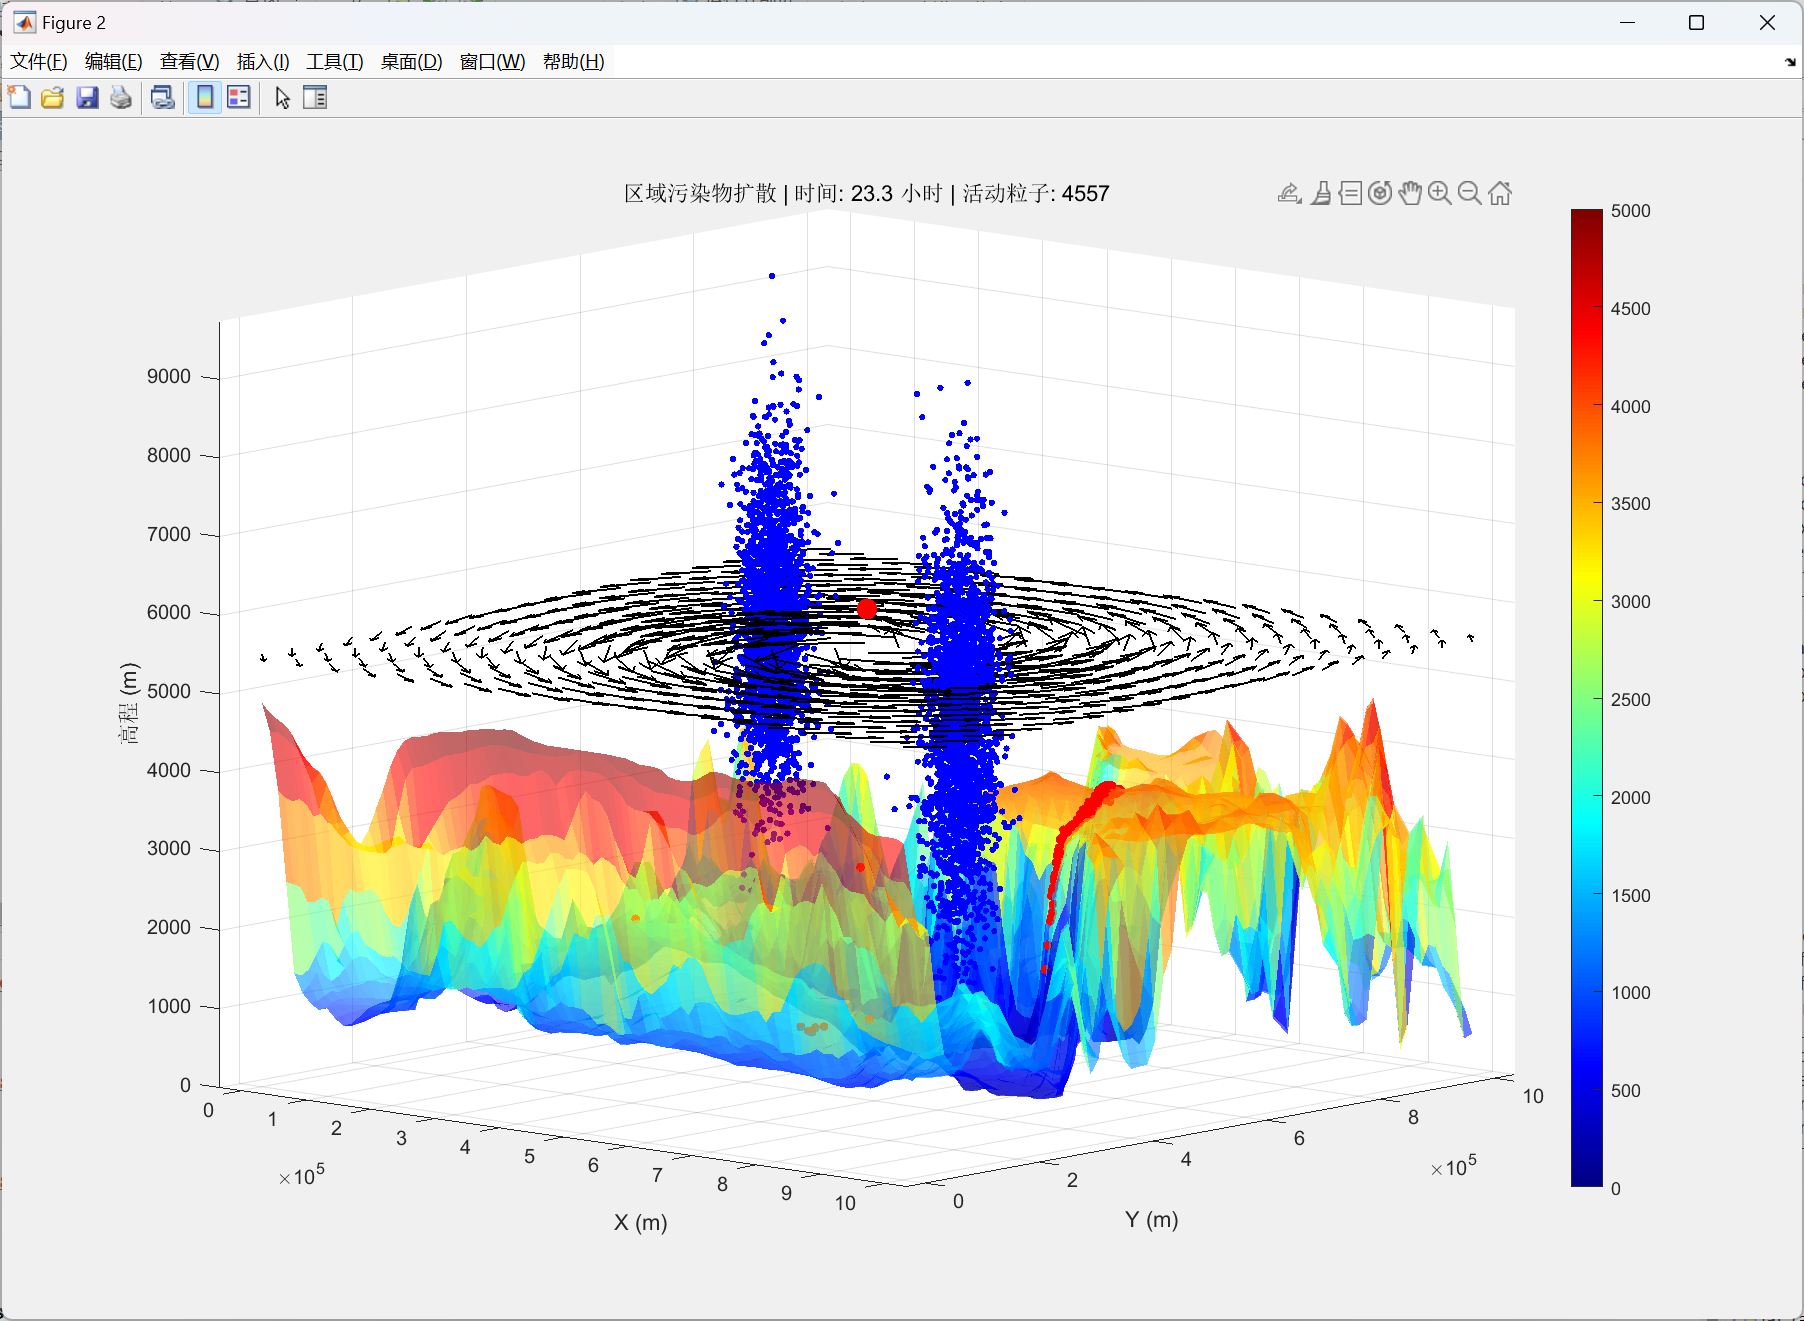
\includegraphics[width=10cm]{Lagrange3.png}
		\caption{扩散后期分布图2}
		\label{fig:your_label}
	\end{figure}
	\FloatBarrier
	\newpage
	\subsection{稳态下的高斯烟羽模型}
	\begin{figure}[htbp]
		\centering
		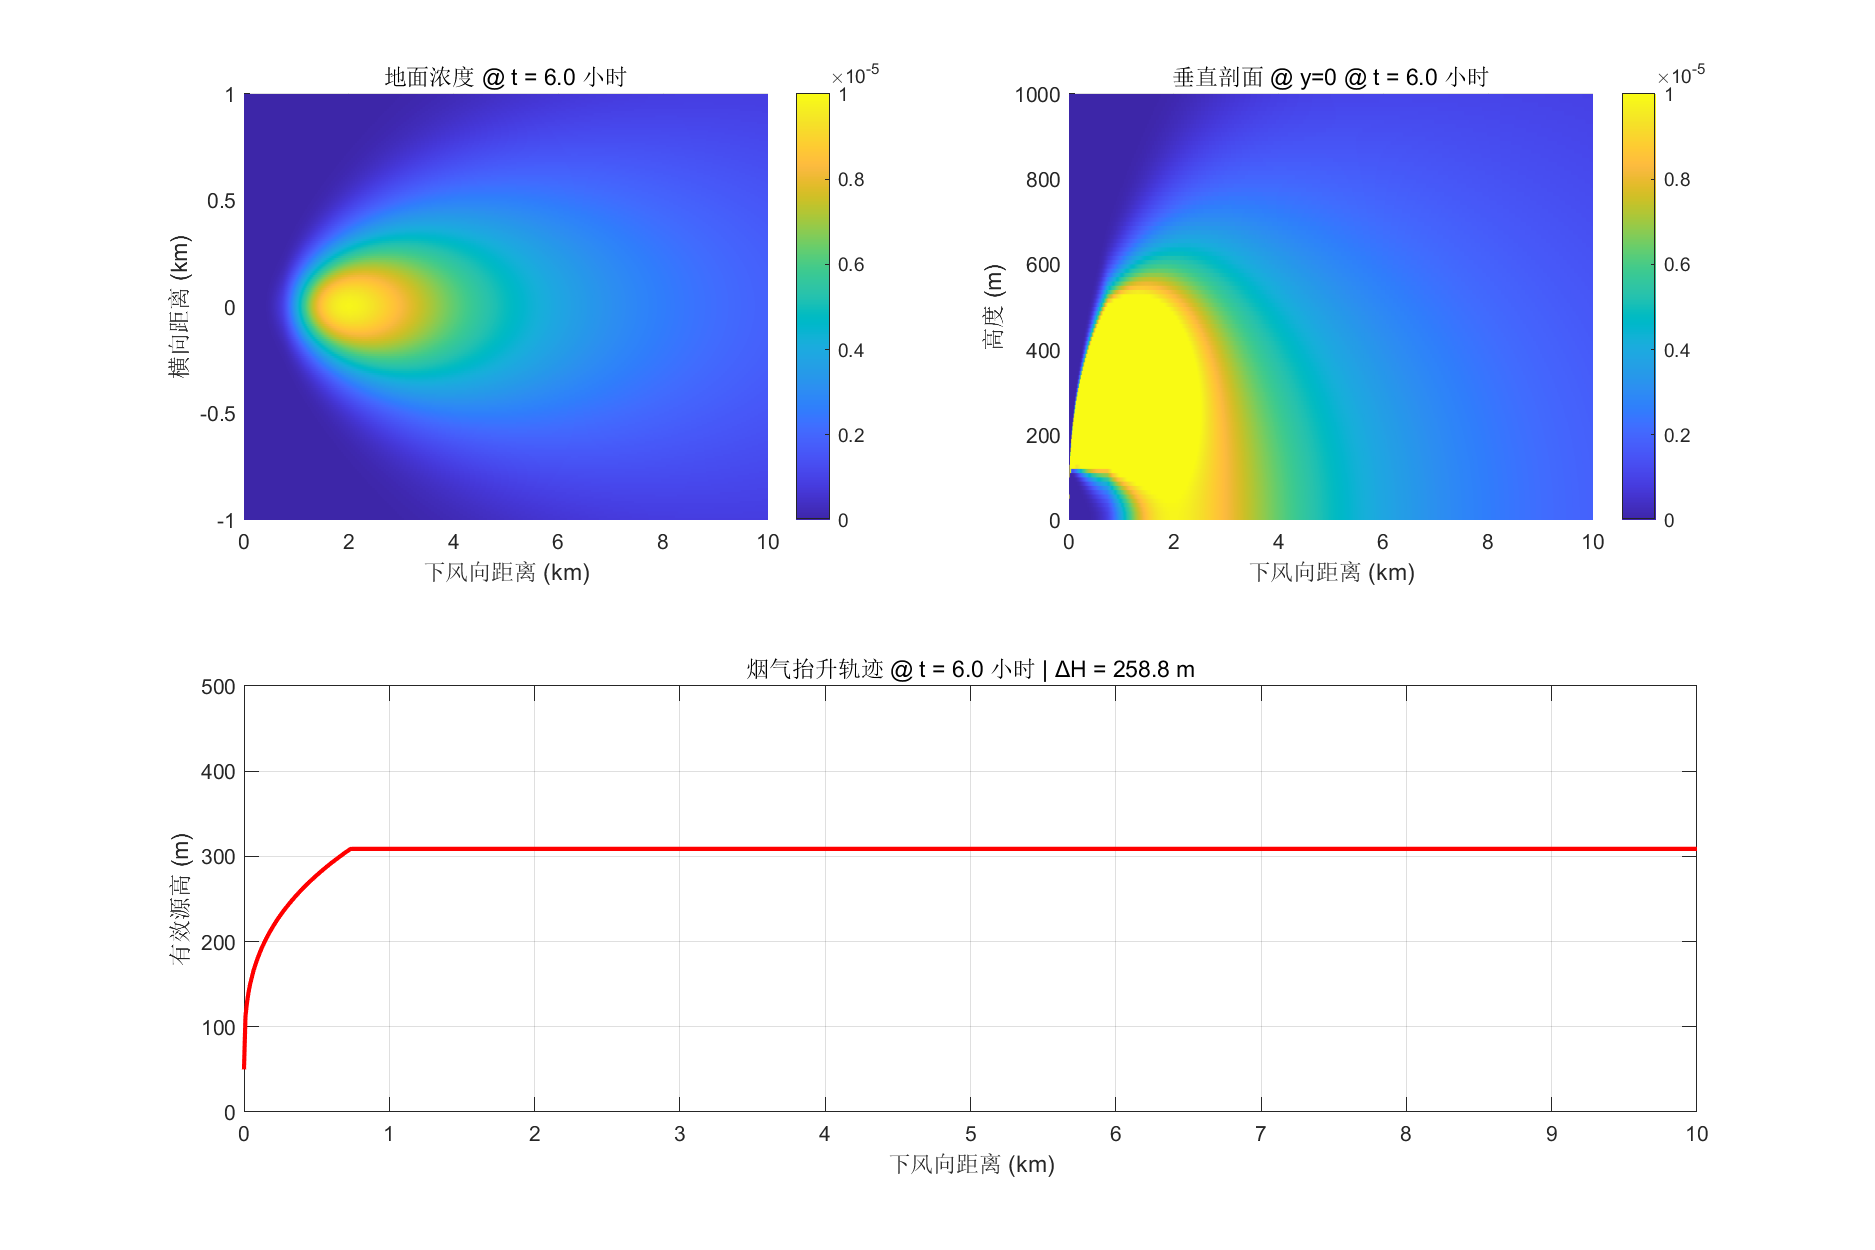
\includegraphics[width=15cm]{gauss.png}
		\caption{高斯烟羽模型}
		\label{fig:your_label}
	\end{figure}
	
	
		\setcounter{section}{5}
	\setcounter{subsection}{0}
	\section*{\centerline{五、结论}}
	\indent 本实验基于拉格朗日粒子模型与高斯烟羽模型,分别在不同风场与地形条件下对大气污染物(PM2.5)的扩散行为进行了模拟与分析。通过对比不同模型下的扩散形态和沉积分布,得到如下结论
	\subsection{模型适用性}
	\begin{itemize}
		\item 高斯烟羽模型适用于稳态、匀速风场下的污染物扩散模拟,计算效率高,适用于快速估算和初步评估。
		\item 拉格朗日粒子模型更适用于描述复杂、非稳态风场与复杂地形条件下的污染物扩散,具有更强的灵活性和精度,但计算量较大。
	\end{itemize}
	\subsection{风场对扩散的影响}
	\begin{itemize}
		\item 在匀速风场中,污染物呈现烟羽状扩散,符合高斯分布特征。
		\item 在旋转风场中,污染物呈现螺旋状扩散轨迹,显示出明显的旋转对流特性
		\item 外力因素对粒子扩散的影响远大于其本身的布朗运动
	\end{itemize}
	\subsection{地形对扩散的影响}
	\begin{itemize}
		\item 复杂地形显著影响粒子的沉积分布,地势起伏较大的区域更易形成污染物的堆积。
	\end{itemize}
	\section*{\centerline{六、问题}}
	\indent 在追踪大量粒子时,拉格朗日模型的计算复杂度较高,运行时间较长,可以考虑使用并行算法等优化方式提升效率。相对的,高斯烟羽模型尽管计算效率高,但在非稳态或复杂地形下误差较大,可以考虑构建半解析模型等方式进行改进。除此之外,粒子在与地面碰撞之后的状态用简单的按比例沉积与反弹误差过大,实际上这与地面各种特性,温度等均有关联。以及影响粒子运动的因素还有很多,地形对扩散的影响也要更为复杂,可以在未来考虑更多的因素来增加数学模型的准确性,使其更具价值。展示方面,目前的三维动态可视化过程相对简陋,结果展示方面也不够直观明显,优化这一部分的算法也可以提升结果质量。
	
	
	

	
	\begin{table}[htbp]
		\caption{\textbf{符号说明}}%标题
		\centering%把表居中
		\begin{tabular}{ccc}%内容全部居中
			\toprule%第一道横线
			符号&说明&单位 \\
			\midrule%第二道横线 
			$\vec{X}(t)$ & 粒子在$t$时刻所处的位置向量&  $m$\\
			$\vec{U}(t)$ & $t$时刻$\vec{X}$位置的环境风场 &  $m/s$\\
			$\vec{R}(t)$ & $t$时刻湍流扰动 & $m/s$\\
			$C(x,y,z)$   & 污染物在$(x,y,z)$处的浓度 &$g/m^3$ \\
			$Q$          & 源强 & $g/m$ \\
			$H$          &有效排放距离 &$m$\\
			$ \sigma_y,\sigma_z $& 扩散系数 &  \\
			$u_*$ 磨擦速度&  $m/s$\\
			$\kappa$     &von Kármán常数&  \\
			$d$          & 地表障碍物高度 & $m$\\
			$z_0$         & 地面粗糙度长度 &  $m$\\
			\bottomrule%第三道横线
			
			
		\end{tabular}
	\end{table}
	
	\nocite{pasquill1961estimation}
	\nocite{draxler1997description}
	\bibliographystyle{ieeetr}
	\bibliography{refer}
	
\end{document}
